This chapter discusses the continuous-time Fourier transform. We'll cover the following topics:
\begin{itemize}
    \item Important Fourier transform pairs
    \item Plancherel's theorem and Parseval's theorem 
    \item Convolution theorem
    \item Impulse response and frequency response of LTI systems
    \item Fourier transform of a time shifted signal
\end{itemize}

\noindent The \emph{\index{forward Fourier transform}{forward Fourier transform}} is defined as:
\begin{equation}
\boxed{
\hat{x}(\omega) = \int_{-\infty}^{\infty} x(t) e^{-i\omega t}dt}
\end{equation}
and the \emph{\index{inverse Fourier transform}{inverse Fourier transform}} is defined as:
\begin{equation}
\boxed{
x(t) = \frac{1}{2\pi}\int_{-\infty}^{\infty} \hat{x}(\omega) e^{i\omega t}d\omega\,\,.
}
\end{equation}
We'll use the following notation to indicate Fourier transform pairs:
\begin{equation}
\boxed{x(t) \xleftrightarrow{\mathcal{F}} \hat{x}(\omega)\,\,.}
\end{equation}
The left denotes the \emph{\index{time domain}{time domain}} representation of the signal and the right-hand side denotes the \emph{\index{frequency domain}{frequency domain}} representation of the same signal. I've used a hat to signify that the symbol $\hat{x}(\omega)$ is a frequency domain representation of a signal.

The existence or non-existence of a Fourier transform or an inverse Fourier transform is rarely something that is encountered in signal processing applications. Exploring this topic rigorously is outside the scope of this course.

\section{Selected Fourier transform}
It is impossible to exhaustively cover all of the possible Fourier transform pairs here. We'll only give examples of commonly encountered Fourier transforms and provide solution strategies for using these as basic building blocks to evaluate the Fourier transform for more complicated signals. Refer to a formula book\sidenote{The wikipedia article also contains a nice table of Fourier transform pairs:\url{https://en.wikipedia.org/wiki/Fourier_transform}.}\cite{kammler2007firs} for a more complete table of Fourier transform pairs.

\subsection{Linear combination}
The Fourier transform of a linear combination of signals in time domain is related to a linear combination of Fourier transforms in frequency domain:
\begin{equation}
\boxed{
y(t)=c_1 x_1(t)  + c_2 x_2(t) \xleftrightarrow{\mathcal{F}} \hat{y}(\omega) = c_1\hat{x}_1(\omega)+c_2\hat{x}_2(\omega)\,\,.
}
\end{equation}
This is can be shown as follows:
\begin{align}
\hat{y}(\omega) &= \int_{-\infty}^{\infty} [c_1 x_1(t)+c_2 x_2(t)] e^{-i\omega t} dt \\
&= c_1\int_{-\infty}^{\infty} x_1(t) e^{-i\omega t} dt + c_2\int_{-\infty}^{\infty} x_2(t) e^{-i\omega t} dt \\ 
&=  c_1\hat{x}_1(\omega)+c_2\hat{x}_2(\omega)\qed\,\,.
\end{align}
This may seem trivial, but keep this property in mind, as it can be used to Fourier transform more complicated signals that are a superposition of simple individual signals.


\subsection{Fourier transform of $\delta(t+\tau)$}

\begin{marginfigure}
\begin{center}
        \begin{tikzpicture}
        \begin{axis}[width=6cm,height=4cm,ymin=0,xmin=0,ymax=1.1,xmax=2,         
        yticklabels={,,},
        xtick={1},
        ytick={0},
        xticklabels={$-\tau$},
        xlabel=$t$,
        ylabel={$x(t)=\delta(t+\tau)$}, 
        axis lines = center]

\addplot +[dirac] coordinates {(1,0.8)};
%\node at (axis cs:1.25,1) [below, font={\footnotesize}]{$\delta(t+\tau)$};

\end{axis}
        \end{tikzpicture}

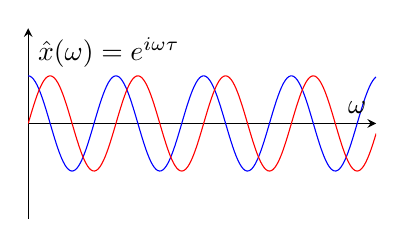
\begin{tikzpicture}
	\begin{axis}[domain=0:(2*6.23),
        width=6cm,
        height=4cm,
        ticks=none,
        axis lines = center,
        ymax=2,
        ymin=-2,
        samples=200,
        legend pos=north east,
        legend style={draw=none},
        xlabel={$\omega$},
        ylabel={$\hat{x}(\omega)=e^{i\omega \tau}$}]
    \addplot[blue] {cos(2*deg(x))};
    \addplot[red] {sin(2*deg(x))};
%    \node at (axis cs:3.14,-1.5) {$\displaystyle{T=\frac{2\pi}{\omega}}$};   
%    \addplot [dimen] plot coordinates {(1.57,-1.1) (4.71,-1.1)};   
%    \legend{$\mathrm{Re}(e^{i\omega t})$,$\mathrm{Im}(e^{i\omega t})$}
    \end{axis}
\end{tikzpicture}
\end{center}
\caption{Unit impulse signal $\delta(t+\tau)$ is non-zero only when $t=-\tau$. In frequency domain, the Fourier transform is a complex sinusoidal signal with $\omega$ the independent variable.}
\end{marginfigure}


The time shifted unit impulse signal is a complex sinusoidal signal in frequency domain:
\begin{equation}
\boxed{
  x(t)=\delta(t+\tau) \xleftrightarrow{\mathcal{F}} \hat{x}(\omega) = e^{i\omega \tau}\,\,.
  \label{eq:fttss}
}
\end{equation}
This is also relatively easy to show:
\begin{align}
\hat{x}(\omega) &= \int_{-\infty}^{\infty} x(t) e^{-i\omega t} dt \\
&= \int_{-\infty}^{\infty} \delta(t+\tau) e^{-i\omega t} dt \\
&= e^{i\omega \tau} \qed\,\,.
\end{align}

\subsection{Fourier transform of $e^{i\omega_0 t}$}


\begin{marginfigure}
\begin{center}

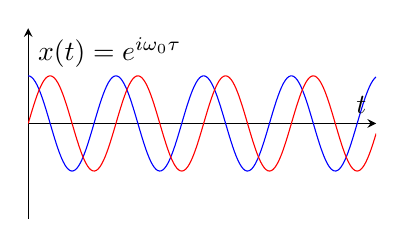
\begin{tikzpicture}
\begin{axis}[domain=0:(2*6.23),
        width=6cm,
        height=4cm,
        ticks=none,
        axis lines = center,
        ymax=2,
        ymin=-2,
        samples=200,
        legend pos=north east,
        legend style={draw=none},
        xlabel={$t$},
        ylabel={$x(t) =e^{i\omega_0 \tau}$}]
    \addplot[blue] {cos(2*deg(x))};
    \addplot[red] {sin(2*deg(x))};
    \end{axis}
\end{tikzpicture}

\begin{tikzpicture}
        \begin{axis}[width=6cm,height=4cm,ymin=0,xmin=0,ymax=1.1,xmax=2,         
        yticklabels={,,},
        xtick={1},
        ytick={0},
        xticklabels={$\omega_0$},
        xlabel=$\omega$,
        ylabel={$\hat{x}(\omega)=2\pi \delta(\omega-\omega_0)$}, 
        axis lines = center]

\addplot +[dirac] coordinates {(1,0.8)};
\end{axis}
\end{tikzpicture}
\end{center}
\caption{A complex sinusoidal signal of frequency $\omega_0$ is a unit impulse signal $\delta(\omega-\omega_0)$ in frequency domain.}
\end{marginfigure}

The converse of the previous is a complex sinusoidal signal $e^{i\omega_0 t}$ with frequency $\omega_0$. This has the following Fourier transform pair:
\begin{equation}
\boxed{
x(t) = e^{i\omega_0 t} \xleftrightarrow{\mathcal{F}} \hat{x}(\omega) = 2\pi \delta(\omega-\omega_0)\,\,.
}
\end{equation}
We show this by inverse Fourier transforming $\hat{x}(\omega)$:
\begin{align}
x(t) &= \frac{1}{2\pi}\int_{-\infty}^{\infty} \hat{x}(\omega) e^{i\omega t} d\omega \\
 &= \frac{1}{2\pi}\int_{-\infty}^{\infty} 2\pi \delta(\omega-\omega_0)e^{i\omega t} d\omega \\
 &= e^{i\omega_0 t}\qed\,\,.
\end{align}

\subsection{Rectangular function}
One often encountered Fourier transform pair is that of the rectangular function\footnote{Also often called the boxcar function.} of length $T$:
\begin{equation}
\boxed{
x(t)=u\left(t+\frac{T}{2}\right) - u\left(t-\frac{T}{2}\right) \xleftrightarrow{\mathcal{F}} \hat{x}(\omega) = \frac{1}{i\omega}(e^{i\omega \frac{T}{2}} - e^{-i\omega \frac{T}{2}})\,\,.
}
\end{equation}

This can be derived as follows:
\begin{align}
\hat{x}(\omega) &= \int_{-\infty}^{\infty} \left[u\left(t+\frac{T}{2}\right) - u\left(t-\frac{T}{2}\right)\right] e^{-i\omega t}dt \\
&= \int_{-T/2}^{T/2} e^{-i\omega t}dt\\
&=  \left.-\frac{e^{-i\omega t}}{i\omega} \right|_{t=-T/2}^{T/2}\\
&= \frac{e^{i\omega \frac{T}{2}}- e^{-i\omega \frac{T}{2}}}{i\omega}\,\,.
\end{align}
We can use Euler $\sin(x) = \frac{1}{2i} (e^{i x} - e^{-ix})$ to express this as follows:

\begin{marginfigure}
\begin{center}

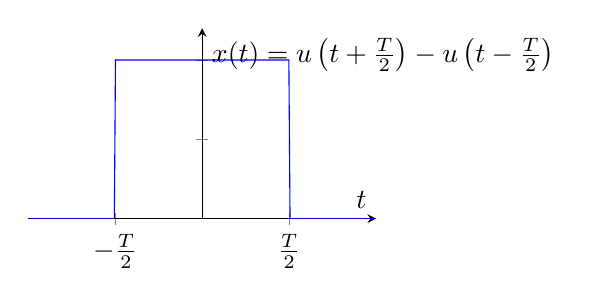
\begin{tikzpicture}
	\begin{axis}[domain=(-1):(1),samples=300,
        width=6cm,
        height=4cm,
    ymin=0,ymax=1.2,
        xlabel={$t$},
        ylabel={$x(t)=u\left(t+\frac{T}{2}\right) - u\left(t-\frac{T}{2}\right)$},
        axis x line=center, 
        axis y line=center, 
        yticklabels={,,,}, 
        xtick={-0.5,0.5},
        xticklabels={$-\frac{T}{2}$,$\frac{T}{2}$}
    ]

    \addplot[blue] {(x>-0.5)*(x<0.5)};
\end{axis}
\end{tikzpicture}

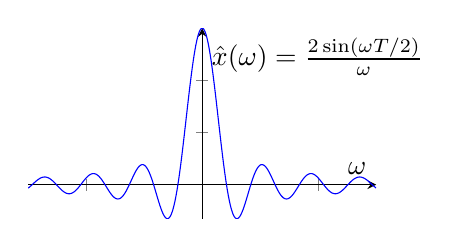
\begin{tikzpicture}
	\begin{axis}[domain=(-15):(15),samples=300,
        width=6cm,
        height=4cm,        
        xlabel={$\omega$},
        ylabel={$\hat{x}(\omega)=\frac{2\sin(\omega T/2)}{\omega}$},
        axis x line=center, 
        axis y line=center, 
        yticklabels={,,,}, 
        xticklabels={,,,}
    ]
    \addplot[blue] {2*sin(0.5*3*deg(x))/x};
\end{axis}
\end{tikzpicture}
\end{center}
\caption{The Fourier transform of a boxcar function.}
\end{marginfigure}

\begin{equation}
\boxed{
\hat{x}(\omega) = \frac{2\sin(\omega \frac{T}{2})}{\omega}\,\,.
}
\end{equation}
The function $\mathrm{sinc}(\omega)=\sin(\pi\omega)/(\pi\omega)$ is often used to express this function. This is convenient, as numerical implementations (such as \verb|numpy.sinc|) of the function deal with the special case when $\omega=0$, which can be investigated using L'H\^{o}pital's rule:
\begin{equation}
\lim_{\omega \rightarrow c} \frac{f(\omega)}{g(\omega)} = \lim_{\omega \rightarrow c} \frac{f'(\omega)}{g'(\omega)}\,\,.
\end{equation}
Which in this case is:
\begin{equation}
\lim_{\omega \rightarrow 0} \frac{2\sin(\omega T/2)}{\omega} = \lim_{\omega \rightarrow 0} T\cos(\omega T/2 ) = T\,\,.
\end{equation}
We'll be using L'H\^{o}pital's rule elsewhere in signal processing to resolve similar situations.

\subsection{Sinc function}
A related Fourier transform pair is the one where the frequency domain representation is a rectangular function. This is used e.g., when calculating ideal filters. This result is also used in Shannon's sampling theorem to obtain an ideal reconstruction filter for band limited signals that only have spectral components in the band
$|\omega| < \omega_b$.
\begin{equation}
\boxed{
x(t) = \frac{\sin(\omega_b t)}{\pi t} \xleftrightarrow{\mathcal{F}} \hat{x}(\omega) = u(\omega+\omega_b) - u(\omega-\omega_b)\,\,.
}
\label{eq:ft:sinc}
\end{equation}
This relationship can be shown by inverse Fourier transforming $\hat{x}(\omega)$:
\begin{align}
x(t) &= \frac{1}{2\pi}\int_{-\infty}^{\infty} \left[u(\omega+\omega_b) - u(\omega-\omega_b)\right] e^{i\omega t}d\omega \\
 &= \frac{1}{2\pi}\int_{-\omega_b}^{\omega_b} e^{i\omega t}d\omega \\
 &= \frac{1}{2\pi}\left.\frac{e^{i\omega t}}{it}\right|_{\omega=-\omega_b}^{\omega_b} \\
 &= \frac{e^{i t \omega_b} - e^{-i t \omega_b} }{ 2\pi i t} \\
 &= \frac{\sin(\omega_b t)}{\pi t}\qed\,\,.
\end{align}
Fourier transforming the sinc-function is not as trivial.

\begin{marginfigure}
\begin{center}
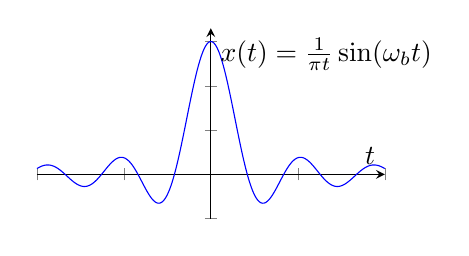
\begin{tikzpicture}
	\begin{axis}[
        width=6cm,
        height=4cm,
        domain=(-10):(10),
        samples=300,
        ymin=-1,
        ymax=3.3,
        xlabel={$t$},
        ylabel={$x(t)=\frac{1}{\pi t}\sin(\omega_b t)$},
        axis x line=center, 
        axis y line=center, 
        yticklabels={,,,}, 
        xticklabels={,,,}
    ]
    \addplot[blue] {2*sin(0.5*3*deg(x))/x};
\end{axis}
\end{tikzpicture}

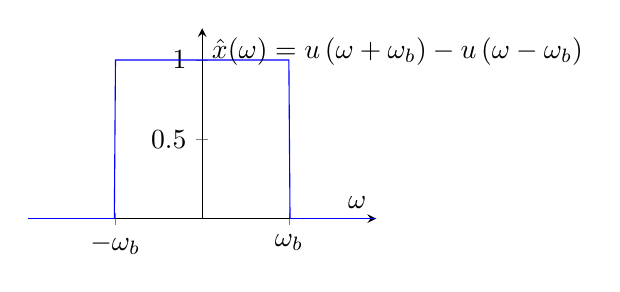
\begin{tikzpicture}
	\begin{axis}[
        width=6cm,
        height=4cm,
        domain=(-1):(1),
        samples=300,
        ymin=0,
        ymax=1.2,
        xlabel={$\omega$},
        ylabel={$\hat{x}(\omega) = u\left(\omega+\omega_b\right) - u\left(\omega-\omega_b\right)$},
        axis x line=center, 
        axis y line=center, 
        xtick={-0.5,0.5},
        xticklabels={$-\omega_b$,$\omega_b$}
    ]
    \addplot[blue] {(x>-0.5)*(x<0.5)};
\end{axis}
\end{tikzpicture}
\end{center}
\caption{A sinc function in time domain is a boxcar function in frequency domain.}
\end{marginfigure}

\subsection{Gaussian}
The Fourier transform of a Gaussian density function is another Gaussian density function:
\begin{equation}
\boxed{x(t) = e^{-\alpha t^2} \xleftrightarrow{\mathcal{F}} \sqrt{\frac{\pi}{\alpha}} e^{-\frac{\omega^2}{4\alpha}}\,\,.}
\end{equation} 
Note that the width of the time domain Gaussian is inversely proportional to the width of the frequency domain Gaussian.

If we rewrite the above into a form which resembles a Gaussian density function normalized to unity at zero, with a width parameter $\sigma_t$ and $\sigma_\omega$ for the time domain and frequency domain width, we get:
% 4*a = 1/2s**2.0
\begin{equation}
x(t) \propto e^{-\frac{t^2}{2\sigma_t^2}} \xleftrightarrow{\mathcal{F}} \hat{x}(\omega) \propto e^{-\frac{\omega^2}{2\sigma_\omega^2}}\,\,,
\end{equation}
which implies that:
\begin{equation}
\frac{1}{\sigma_t} = \sigma_\omega\,\,.
\end{equation}%$\alpha=(1/2)*s_t^2$
This is a very nice demonstration of the inverse relationship between the width of a signal in time domain and frequency domain. When we discuss filters later on, we'll use this to show that the length of a filter in time domain is inversely proportional to the spectral resolution (width of the filter response).

\begin{marginfigure}
\begin{center}
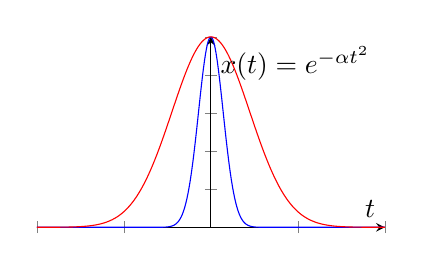
\begin{tikzpicture}
	\begin{axis}[
        width=6cm,
        height=4cm,
        domain=(-10):(10),
        samples=300,
        xlabel={$t$},
        ylabel={$x(t)=e^{-\alpha t^2}$},
        axis x line=center, 
        axis y line=center, 
        yticklabels={,,,}, 
        xticklabels={,,,}
    ]
    \addplot[blue] {exp(-x*x)};
        \addplot[red] {exp(-0.1*x*x)};

\end{axis}
\end{tikzpicture}

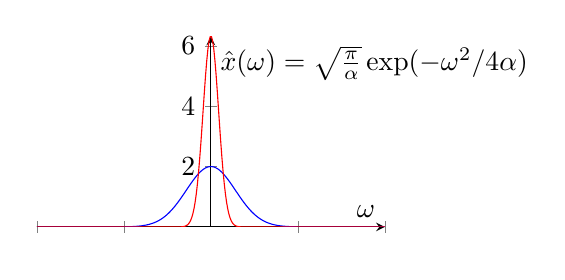
\begin{tikzpicture}
	\begin{axis}[
        width=6cm,
        height=4cm,
        domain=(-10):(10),
        samples=300,
        xlabel={$\omega$},
        ylabel={$\hat{x}(\omega) = \sqrt{\frac{\pi}{\alpha}}\exp(-\omega^2/4\alpha)$},
        axis x line=center, 
        axis y line=center, 
        xticklabels={,,,}
    ]
    \addplot[blue] { sqrt(4)*exp(-x*x/4)) };
        \addplot[red] { sqrt(4/0.1)*exp(-x*x/(4*0.1))) };
\end{axis}
\end{tikzpicture}
\end{center}
\caption{The Fourier transform of a Gaussian density function is another Gaussian density function. The width of the frequency domain and time domain density functions are inversely proportional.}
\label{fig:gaussftf}
\end{marginfigure}

This Fourier transform pair can be derived as follows:
\begin{align}
\hat{x}(\omega) &= \int_{-\infty}^{\infty} e^{-\alpha t^2} e^{-i\omega t} dt \\
&= \int_{-\infty}^{\infty} e^{-\alpha t^2 - i\omega t} dt\,\,.
\end{align}
We perform a little trick and multiply with $1=e^{c^2\omega^2}e^{-c^2\omega^2}$ using a procedure called completing the square, so that we can get to a variable substitution that allows us to easily integrate the function inside the integral:
\begin{align}
\hat{x}(\omega) &= e^{c^2 \omega^2}\int_{-\infty}^{\infty} e^{-\alpha t^2 -i\omega t - c^2 \omega^2} dt\,\,.
\end{align}
We now substitute a variable $\alpha'=\sqrt{\alpha}$. We then need to find a constant $c$ so that:
\begin{equation}
-t^2\alpha'^2 - i\omega t - c^2 \omega^2 = -(t \alpha' + c\omega)^2\,\,.
\end{equation}
We find that $c=\frac{i}{2\alpha'}$.% t**2a**2 + 2*t*a*c*o + c**2*o**2, c = i/(2a)
\begin{equation}
\hat{x}(\omega) = e^{-\frac{\omega^2}{4\alpha}} \int_{-\infty}^{\infty} e^{-\left(t\alpha' + \frac{i}{2\alpha'}\omega\right)^2} dt\,\,.
\end{equation}
Now we perform a variable substitution: $u=t\alpha' + \frac{i}{2\alpha'}\omega$, which gives us: $\frac{1}{\alpha'}du = dt$. 

We now need to refer to a table of integrals to obtain a solution to the integral:
\begin{align}
\int_{-\infty}^{\infty} e^{-u^2} du &= \sqrt{\pi}
\end{align}
and thus
\begin{align}
\hat{x}(\omega) &= \frac{1}{\sqrt{\alpha}}e^{-\frac{\omega^2}{4\alpha}} \int_{-\infty}^{\infty} e^{-u^2} du\\
&=\sqrt{\frac{\pi}{\alpha}} e^{-\frac{\omega^2}{4\alpha}}\,\,.
\end{align}
The plots in Figure \ref{fig:gaussftf} show the time domain and frequency domain Fourier transform pairs for two different values of $\alpha$, which demonstrates the inverse relationship between the width of the function in time and frequency domain.

\subsection{Exponentially decaying signal $x(t) = e^{-\beta t}u(t)$}

\begin{marginfigure}
\begin{center}
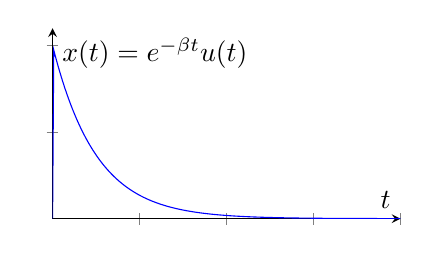
\begin{tikzpicture}
	\begin{axis}[domain=(0):(4),samples=300,
                width=6cm,
        height=4cm,
    ymin=0,ymax=1.1,
        xlabel={$t$},
        ylabel={$x(t)=e^{-\beta t} u(t)$},
        axis x line=center, 
        axis y line=center, 
        yticklabels={,,,}, 
        xticklabels={,,,}
    ]
    \addplot[blue] {(x>0)*exp(-2*x)};
\end{axis}
\end{tikzpicture}

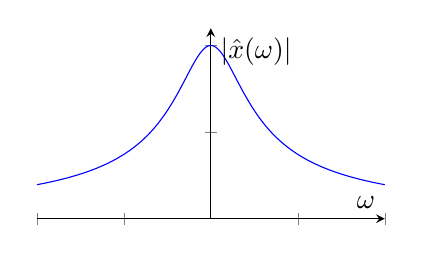
\begin{tikzpicture}
	\begin{axis}[domain=(-10):(10),samples=300,
        width=6cm,
        height=4cm,
    ymin=0,ymax=1.1,
        xlabel={$\omega$},
        ylabel={$|\hat{x}(\omega)|$},
        axis x line=center, 
        axis y line=center, 
        yticklabels={,,,}, 
        xticklabels={,,,}
    ]
    \addplot[blue] {abs(2/sqrt(4+x*x))};
\end{axis}
\end{tikzpicture}

\end{center}
\caption{The Fourier transform of an exponentially decaying signal.}
\end{marginfigure}

When $\beta \in \mathbb{R}_{>0}$ the signal $e^{-\beta t} u(t)$ decays exponentially. This type of signal is often encountered in electrical circuits (e.g., a low pass filter) and in control systems:
\begin{equation}
\boxed{x(t)=e^{-\beta t} u(t) \xleftrightarrow{\mathcal{F}} \hat{x}(\omega)=\frac{1}{\beta + i\omega}\,\,.}
\end{equation}
This can be derived as follows:
\begin{align}
\hat{x}(\omega) &= \int_{-\infty}^{\infty} e^{-\beta t} u(t) e^{-i\omega t}dt \\
&= \int_{0}^{\infty} e^{-(\beta+i\omega) t} dt \\
&= \left. -\frac{1}{\beta + i\omega} e^{-(\beta + i\omega)t} \right|_{t=0}^{\infty}\\
&= \frac{1}{\beta + i\omega}\,\,.
\end{align}
The above requires that $\beta \in \mathbb{R}_{> 0}$.

\subsection{Real valued signals}
There is a special conjugate symmetry for signals that are real valued either in time domain or frequency domain. 

If the time domain signal is real valued, then the frequency domain representation is conjugate symmetric.
\begin{equation}
\boxed{
x(t) \in \mathbb{R} \xleftrightarrow{\mathcal{F}} \hat{x}(-\omega)=\hat{x}^*(\omega)\,\,.
}
\end{equation}
The same also applies the other way around. If the spectral representation is real-valued, then the time domain representation is conjugate symmetric:
\begin{equation}
\boxed{
x(-t)=x^*(t) \xleftrightarrow{\mathcal{F}} \hat{x}(\omega) \in \mathbb{R}\,\,.
}
\end{equation}
This can be shown as follows:
\begin{proof}
\begin{align}
\hat{x}^*(\omega) &= \left(\int_{-\infty}^{\infty} x(t) e^{-i\omega t}dt\right)^* \\
 &= \int_{-\infty}^{\infty} x^*(t) e^{i\omega t}dt \\
 &= \int_{-\infty}^{\infty} x(t) e^{i\omega t}dt \\
 &= \hat{x}(-\omega)\,\,.
\end{align}
\end{proof}
Because $x(t)\in\mathbb{R}$, we have that $x^*(t)=x(t)$. A similar proof exists for the real-valued spectral representation. 
% This same property exists for all the spectral representations.

\subsection{Fourier series}
A Fourier series can be used to represent a periodic function as a sum of frequency components. Because we know that the Fourier transform of $e^{i\omega' t}$ is $2\pi\delta(\omega-\omega')$, we can easily determine the Fourier transform of an arbitrary periodic function by using its Fourier series:
\begin{equation}
\boxed{
x(t) = \sum_{k=-\infty}^{\infty} c_k e^{i k \omega_0 t} \xleftrightarrow{\mathcal{F}} \hat{x}(\omega) = 2\pi \sum_{k=-\infty}^{\infty}  c_k \delta(\omega-k\omega_0)\,\,.\label{eq:fsftgen}
}
\end{equation}
The derivation is as follows:
\begin{align}
\hat{x}(\omega) &= \int_{-\infty}^{\infty} \sum_{k=-\infty}^{\infty} c_k e^{ik\omega_0 t} e^{-i\omega t} dt\\
&= \sum_{k=-\infty}^{\infty} c_k\int_{-\infty}^{\infty} e^{ik\omega_0 t}e^{-i\omega t}dt\\
&= 2\pi\sum_{k=-\infty}^{\infty}  c_k \delta(\omega - k\omega_0)\,\,.
\end{align}
This is simply the continuous-frequency representation of Fourier series spectral components. A periodic function has non-zero spectral components only at frequencies that are multiples of $\omega_0$. 
\begin{marginfigure}
\begin{center}
        \begin{tikzpicture}
        \begin{axis}[width=7cm,
        height=6cm,
        ymin=-0,
        xmin=-3,
        ymax=1.8,
        xmax=3,
        yticklabels={,,},
        xtick={-2,-1.5,-1,-0.5,0,0.5,1.0,1.5,2},
        xticklabels={,,},%$-4 \omega_0$,$-3\omega_0$,$-2 \omega_0$,$-\omega_0$,$0$,$ \omega_0$,$2 \omega_0$,$3 \omega_0$,$4 \omega_0$},
    xlabel=$\omega$,
    ylabel=$\hat{x}(\omega)$,
    axis lines = center]
    
   \addplot+[dirac] plot coordinates {(0.5,1) (1.0,0.8) (1.5,0.6) (2,0.5)};
    \addplot+[dirac] plot coordinates {(-0.5,1) (-1.0,0.8) (-1.5,0.6) (-2,0.5)};
   \addplot+[dirac] plot coordinates {(0.0, 1.4)};
    \node at (axis cs:-2.5,0.25) {$\cdots$};   
    \node at (axis cs:2.5,0.25) {$\cdots$};   
    \node at (axis cs:0.25,0.25) {$\omega_0$};   
    
       
    \addplot [dimen] plot coordinates {(0.0,0.35) (0.5,0.35)};

    \node at (axis cs:0.0,1.5) [above right, font={\footnotesize}]{$c_0$};
    \node at (axis cs:0.5,1.1) [above, font={\footnotesize}]{$c_1$};
    \node at (axis cs:1.0,0.9) [above, font={\footnotesize}]{$c_2$};
    \node at (axis cs:1.5,0.7) [above, font={\footnotesize}]{$c_3$};
    \node at (axis cs:2.0,0.6) [above, font={\footnotesize}]{$c_4$};

    \node at (axis cs:-0.5,1.1) [above, font={\footnotesize}]{$c_{-1}$};
    \node at (axis cs:-1.0,0.9) [above, font={\footnotesize}]{$c_{-2}$};
    \node at (axis cs:-1.5,0.7) [above, font={\footnotesize}]{$c_{-3}$};
    \node at (axis cs:-2.0,0.6) [above, font={\footnotesize}]{$c_{-4}$};
\end{axis}
        \end{tikzpicture}
\end{center}
\caption{The Fourier transform of a Fourier series. The spectral representation is a set of spectral lines spaced apart by $\omega_0$, the fundamental angular frequency of the periodic signal. A set of spectral lines spaced apart by a constant value is a spectral signature of a time-periodic signal.}
\end{marginfigure}

\begin{marginfigure}
\begin{center}
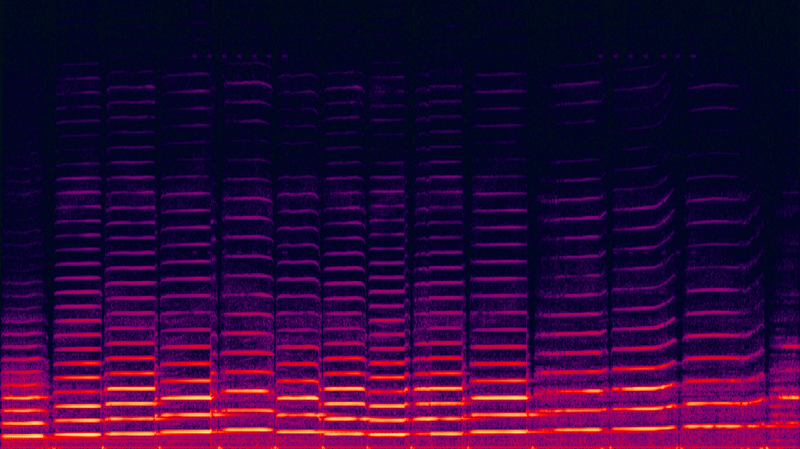
\includegraphics[width=\textwidth]{ch08/figures/real_spectrum.png}
\end{center}
\caption{A time-frequency-power image of a violin being played. The x-axis represents time and the y-axis represents frequency. Only positive frequencies are shown. At any given moment, a violin is playing approximately a time-periodic signal (a single note).  The spectrum is a forest of spectral lines spaced apart by the fundamental angular frequency of the signal.  Credits: Wikipedia.}
\end{marginfigure}

The inverse Fourier transform of the spectrum $\hat{x}(\omega)$ is:
\begin{align}
x(t) &= \frac{1}{2\pi}\int_{-\infty}^{\infty} \hat{x}(\omega)e^{i\omega t} d\omega \\
&= \sum_{k=-\infty}^{\infty} c_k \int_{-\infty}^{\infty} \delta(\omega - k\omega_0) e^{i\omega t} d\omega \\
&= \sum_{k=-\infty}^{\infty} c_k e^{ik\omega_0 t}\,\,.
\end{align}
The fact that the continuous-time Fourier transform and the Fourier series are related in this way shouldn't be too surprising, as we earlier derived the Fourier transform from the Fourier series representation for a periodic function with an infinitely long fundamental period.

\subsection{Time scaling system}
Let's look at a time scaling system:
\begin{equation}
y(t) = x(at)\,\,.
\end{equation}
What effect does this system have on the frequency domain representation of this signal?

We assume that a signal $x(t)$ has a Fourier transform:
\begin{align}
x(t) \xleftrightarrow{\mathcal{F}} \hat{x}(\omega)\,\,.
\end{align}
If we scale the time parameter $x(at)$, then the spectral representation is scaled inversely in frequency:
\begin{align}
\boxed{
  y(t) = x(at) \xleftrightarrow{\mathcal{F}} \hat{y}(\omega) = \frac{1}{|a|}\hat{x}\left(\frac{\omega}{a}\right)\,\,.
  \label{eq:timescale_ft_pair}
}
\end{align}
What does scaling in time mean?
\begin{itemize}
\item compressing a signal in time with $|a|>1$ will stretch the signal in frequency.
\item stretching a signal in time with $|a|<1$ will compress the signal in frequency. 
\end{itemize}
\begin{proof}
The proof is as follows. Let's investigate the case where $a > 0$ and Fourier transform $y(t)$:
\begin{align}
\hat{y}(\omega) &= \int_{-\infty}^{\infty} y(t) e^{-i\omega t}dt\\
                &= \int_{-\infty}^{\infty} x(at) e^{-i\omega t}dt\,\,.
\end{align}
We do a variable substitution $t'=at$, from which it follows that $dt=\frac{1}{a}dt'$ and 
\begin{align}
\hat{y}(\omega) &= \frac{1}{a}\int_{-\infty}^{\infty} x(t') e^{-i\frac{\omega}{a} t' }dt'\\
 &= \frac{1}{a}\hat{x}\left(\frac{\omega}{a} \right)\,\,.
\end{align}
\end{proof}


%If $a\rightarrow 0$, the $x(at) \rightarrow c$ approaches a constant and $\frac{1}{a}\hat{x}(i\frac{\omega}{a})$ approaches a Dirac-delta $c\delta(\omega)$.

%If $a\rightarrow \infty$, then $x(at)$ is compressed in time and the function $\hat{x}(\omega) \rightarrow $




\subsection{Plancherel's theorem}

Plancherel's theorem states that for any two signals $f(t)$ and $g(t)$ with Fourier transforms $\hat{F}(\omega)$ and $\hat{G}(\omega)$ the following integral is satisfied:
\begin{equation}
\boxed{
\int_{-\infty}^{\infty} f(t) g^*(t) dt = \frac{1}{2\pi} \int_{-\infty}^{\infty}  \hat{F}(\omega)\hat{G}^*(\omega) d\omega\,\,.
}
\end{equation}
This is useful, as we can relate the amount of signal power in time domain to the total amount of power in frequency domain. This theorem has many applications in e.g., the theory of random processes, radio astronomical signal processing, and radar signal processing.


\begin{proof}
The proof is as follows. Consider first the following signal, which is represented using the Dirac delta function in frequency domain:
\begin{equation}
\hat{x}(\omega) = \delta(\omega-\omega')\,\,.
\end{equation}
This has a time domain-representation, which is obtained using the inverse Fourier transform:
\begin{align}
x(t) &= \frac{1}{2\pi} \int_{-\infty}^{\infty} \delta(\omega-\omega')e^{i\omega t}d\omega \\
     &= \frac{1}{2\pi} e^{i\omega' t}\,\,.
\end{align}
Let us now consider the Fourier transform representations for these two signals:
\begin{align}
f(t) &= \frac{1}{2\pi} \int_{-\infty}^{\infty} F(\omega) e^{i\omega t}d\omega \\
g(t) &= \frac{1}{2\pi} \int_{-\infty}^{\infty} G(\omega') e^{i\omega' t}d\omega'\,\,.
\end{align}
If we multiply the Fourier representations of these two and integrate
over time:
\begin{align}
\int_{-\infty}^{\infty} f(t)g^*(t)dt &= \frac{1}{(2\pi)^2} \int_{-\infty}^{\infty}  \left[\int_{-\infty}^{\infty} F(\omega) e^{i\omega t}d\omega \right] \left[ \int_{-\infty}^{\infty} G^*(\omega') e^{-i\omega' t}d\omega' \right]dt\\
&= \frac{1}{(2\pi)^2} \int_{-\infty}^{\infty} F(\omega) \int_{-\infty}^{\infty} G^*(\omega') \int_{-\infty}^{\infty} e^{i(\omega-\omega')t}dt d\omega' d\omega\\
&=\frac{1}{2\pi} \int_{-\infty}^{\infty} F(\omega) \int_{-\infty}^{\infty} G^*(\omega') \delta(\omega-\omega') d\omega' d\omega \\
&=\frac{1}{2\pi} \int_{-\infty}^{\infty} F(\omega) G^*(\omega)  d\omega \,\,.
\end{align}
\end{proof}
The key to this proof is that:
\begin{align}
\int_{-\infty}^{\infty} e^{i(\omega-\omega')t}dt &= \int_{-\infty}^{\infty} e^{-i\omega' t} e^{i\omega t} dt = 2\pi \delta(\omega - \omega')\,\,.
\end{align}


\newthought{Parseval's theorem} is simply a corollary of Plancherel's theorem. If we state that $f(t)=g(t)=x(t)$, then Plancherel's theorem becomes:
\begin{equation}
\boxed{
\int_{-\infty}^{\infty} |x(t)|^2 dt = \frac{1}{2\pi} \int_{-\infty}^{\infty} | \hat{x}(\omega)|^2 d\omega\,\,.
}
\end{equation}
In physics this means that the total energy of the signal in time domain and frequency domain is equivalent, up to a predefined fixed scaling constant. 


\subsection{Convolution theorem}
The convolution theorem states that a convolution operation in time domain is a multiplication operation in frequency domain. A convolution sum of signals $x_1(t)$ and $x_2(t)$ is defined as:
\begin{equation}
\boxed{
x_1(t)*x_2(t) := \int_{-\infty}^{\infty} x_1(\tau) x_2(t-\tau)d\tau\,\,.
}
\end{equation}
The star symbol ($*$) is often used in short hand to express this operation.

An often used property in signal processing is that convolution in time domain is multiplication in frequency domain.
\begin{equation}
\boxed{
y(t) =
x_1(t)*x_2(t) \xleftrightarrow{\mathcal{F}} \hat{y}(\omega)=\hat{x}_1(\omega)\hat{x}_2(\omega)\,\,.
}
\end{equation}



\begin{proof}
\begin{align}
\hat{y}(\omega) &= \int_{-\infty}^{\infty} y(t) e^{-i\omega t} dt \\
                 &= \int_{-\infty}^{\infty} \left( \int_{-\infty}^{\infty} x_1(\tau) x_2(t-\tau) d\tau \right) e^{-i\omega t} dt \\
                 &= \int_{-\infty}^{\infty}   x_1(\tau) \left( \int_{-\infty}^{\infty} x_2(t-\tau) e^{-i\omega t} dt \right) d\tau \,\,.
\end{align}
Next, we perform substitution of variables $m=t-\tau$. From this, it follows that $t=m+\tau$ and $dm=dt$. After substitution, we get:
\begin{align}
\hat{y}(\omega)&= \int_{-\infty}^{\infty}   x_1(\tau) \left( \int_{-\infty}^{\infty} x_2(m) e^{-i\omega m} dm \right) e^{-i\omega \tau} d\tau  \\
                &= \hat{x}_2(\omega) \int_{-\infty}^{\infty}   x_1(\tau)  e^{-i\omega \tau} d\tau  \\
                &= \hat{x}_1(\omega)\hat{x}_2(\omega)\,\,.
\end{align}
\end{proof}
\newthought{The converse of the previous is that multiplication in time domain corresponds to convolution in frequency domain}:
\begin{equation}
\boxed{
y(t) = x_1(t)x_2(t) \xleftrightarrow{\mathcal{F}} \hat{y}(\omega) = \frac{1}{2\pi}\hat{x}_1(\omega) * \hat{x}_2(\omega)\,\,.
}
\end{equation}
\begin{proof}
We start by Fourier transforming $x_1(t)x_2(t)$:
\begin{align}
\hat{y}(\omega) &= \int_{-\infty}^{\infty} x_1(t) x_2(t) e^{-i\omega t} dt \,\,.
\end{align}
We then substitute $x_2(t)$ with it's Fourier transform:
\begin{align}
x_2(t) = \frac{1}{2\pi}\int_{-\infty}^{\infty} \hat{x}_2(\omega') e^{i\omega' t}d\omega'\,\,,
\end{align}
which gives us:
\begin{align}
\hat{y}(\omega) &= \int_{-\infty}^{\infty} x_1(t) \left(\frac{1}{2\pi}\int_{-\infty}^{\infty} \hat{x}_2(\omega') e^{i\omega' t} d\omega' \right) e^{-i\omega t} dt\,\,.
\end{align}
We then swap the order of integration and combine all terms with $t$ inside the innermost integral:
\begin{align}
\hat{y}(\omega)   &= \frac{1}{2\pi} \int_{-\infty}^{\infty} \hat{x}_2(\omega')  \left(\int_{-\infty}^{\infty}  x_1(t) e^{i\omega' t} e^{-i\omega t} dt  \right) d\omega'  \\
    &= \frac{1}{2\pi} \int_{-\infty}^{\infty} \hat{x}_2(\omega')  \left(\int_{-\infty}^{\infty}  x_1(t) e^{-{i(\omega-\omega')t}} dt  \right) d\omega'  \\
    &= \frac{1}{2\pi} \int_{-\infty}^{\infty} \hat{x}_2(\omega')  \hat{x}_1\left(\omega-\omega'\right) d\omega'  \\
    &= \frac{1}{2\pi}\hat{x}_1(\omega )  *\hat{x}_2(\omega)\,\,.
\end{align}
\end{proof}
This property is also very useful. We will use it next to inspect the spectrum of an amplitude modulated signal. This property will also be used when deriving Shannon's sampling theorem.

\section{Time shifted signal}
Assuming that the Fourier transform of $x(t)$ is $\hat{x}(\omega)$, the Fourier transform of a \index{time shifted signal} time shifted signal can be obtained using the following formula:
\begin{equation}
\boxed{y(t) = x(t-t_0) \xleftrightarrow{\mathcal{F}} \hat{y}(\omega)= e^{-i\omega t_0}\hat{x}(\omega)\,\,.}
\label{eq:ft:timeshift}
\end{equation}
\begin{proof}
Left as an exercise for now, we'll prove it later using another approach. 
\end{proof}

\subsection{Alternative definitions and notation}
There are several different notations and slightly different definitions of a Fourier transform that one may encounter in the literature. These mainly vary in how the frequency parameter of spectral representation is scaled and what symbols are used to denote frequency and the imaginary number. The underlying mathematical concepts are the same. 

The spectral representation is sometimes written with an explicit function parameter $i\omega$ instead of $\omega$. Sometimes the hat-notation is not used:
\begin{equation}
\hat{x}(\omega) = \hat{x}(i\omega) = x(\omega)\,\,.
\end{equation}
Commonly used symbols for frequency include $\omega$, $\nu$, $\xi$, $\lambda$, $k$, $l$, and $f$. Also, as usual, the imaginary number $i=\sqrt{-1}$ is sometimes denoted with $j$.

The most common alternative form is the one where the frequency parameter is given scaled to units of cycles per unit of $t$:
\begin{equation}
f = \frac{\omega}{2\pi}\,\,.
\end{equation}
If $t$ is in units of time in seconds, then the units of $f$ would be $1/s$ or hertz. With this frequency parameterization, the transform is unitary (it is norm preserving):
\begin{align}
\hat{x}_1(f) &=  \int_{-\infty}^{\infty} x(t) e^{-i 2\pi f  t}d t\\
x(t) &= \int_{-\infty}^{\infty} \hat{x}_1(f) e^{i 2\pi f t} d f\,\,.
\end{align}
Another commonly used definition for the Fourier transform is one where the forward and reverse transform are scaled symmetrically:
\begin{align}
\hat{x}_2(\omega) &= \frac{1}{\sqrt{2\pi}} \int_{-\infty}^{\infty} x(t) e^{-i\omega t}dt \label{eq:ft_alt_form}\\
x(t) &= \frac{1}{\sqrt{2\pi}} \int_{-\infty}^{\infty} \hat{x}_2(\omega) e^{i\omega t}d\omega\,\,.
\end{align}
Sometimes, the sign convention for the forward and reverse transform is changed:
\begin{align}
\hat{x}_3(\omega) &=  \int_{-\infty}^{\infty} x(t) e^{i\omega t}dt\\
x(t) &= \frac{1}{2\pi} \int_{-\infty}^{\infty} \hat{x}_3(\omega) e^{-i\omega t}d\omega\,\,.
\end{align}
All of these alternative Fourier transform definitions have the same general properties, but the exact equations can differ in scaling constants or in sign of the frequencies. For example, if we were to define the Fourier transform as in equation \ref{eq:ft_alt_form}, the Fourier transform of $x(t)=\delta(t+\tau)$ would be $\hat{x}(\omega)=\frac{1}{\sqrt{2\pi}}e^{i\omega \tau}$, which is slightly different than the result we obtained in Equation \ref{eq:fttss}.

\if 0
The Laplace transform:
\begin{equation}
  F(s) = \int_{-\infty}^{\infty} f(t) e^{-st} dt
\end{equation}
is related to the Fourier transform. When $s=i\omega$, the above integral evaluates to the Fourier transform. We will not discuss this transform further in this course, but it is useful to 
\fi
